\chapter{The Satellite Case}
\label{chap:satellite}

In this chapter, we establish the following result:

\begin{theorem}\label{theorem:satellite}
    Suppose $K$ is a satellite knot satisfying the assumptions of Theorem \ref{thm:main_detection}, that is, there is an isomorphism of bigraded vector spaces
    \[
    \widehat{HFK}(K;\mathbb{F}) \cong \widehat{HFK}(T(2,3) \# T(2,3);\mathbb{F}).
    \]
    Then $K$ is isotopic to $T(2,3) \# T(2,3)$.
\end{theorem}

The argument proceeds in several stages. We first apply Schubert's formula to constrain the Alexander polynomials of the pattern and companion of $K$, forcing both to be trefoils and the algebraic winding number to be one (Lemma \ref{lem:satellite_trefoils_windingnumber_1}). We then invoke the Thurston reducing system framework to classify the canonical reducing curves of the monodromy $h$, isolating two non-trivial possibilities (Case A: $\Sigma_0$ is a pair of pants; Case B: $\Sigma_0$ is genus one with one reducing curve, in Lemma \ref{lem:satellite_CaseACaseB}). For each of these cases, we systematically eliminate sub-cases using a combination of Baldwin-Sivek's classification of periodic outer maps, the fractional Dehn twist coefficient bound of Hedden-Mark, and the Honda-Kazez-Matić right-veering criterion, leaving only the connect-sum of two right-handed trefoils. Finally, we briefly address the degenerate $(2,1)$-cable configuration via a direct Alexander polynomial calculation.

We begin by reviewing the definition of a satellite knot.

Let
\[
P \subset S^1 \times D^2
\]
be a knot in $S^3$ lying non-trivially inside an unknotted solid torus, by which we mean that $P$ is not allowed to be inside a 3-ball in the solid torus, and $P$ is not allowed to be isotopic to the core curve of the solid torus. This knot $P$ is called the \textbf{pattern} of the satellite knot. Fix an embedding
\[
f\colon  S^1 \times D^2 \to S^3.
\]
The satellite knot $K$ is defined to be the knot $f(P)$. The core curve of the solid torus $S^1 \times D^2$ is sent to a knot $C$, which is called the \textbf{companion} of the satellite knot. We will sometimes denote the satellite knot $K$ as $P(C)$.

The \textbf{winding number} of the satellite knot $P(C)$ is the winding number of the pattern inside the solid torus:
\begin{definition}
    Let $K = P(C)$ be a satellite knot, where
    \[
    P \subset V = S^1 \times D^2,
    \]
    an unknotted solid torus. The \textbf{(algebraic) winding number} $w$ of $K$ is the algebraic intersection number of $P$ with a meridional disk of $V$. The \textbf{wrapping number} (or \textbf{geometric winding number}) $m$ of $K$ is the minimum number of geometric intersection points between $P$ with a meridional disk of $V$, where the minimum is taken over all ambient isotopies of $P$ within $V$. It is clear that
    \[
    m \geq |w|.
    \]
\end{definition}

We would like to sometimes consider the pattern $P$ as a knot in $S^3$, by which we mean the image of $P$ under the natural embedding of $S^1 \times D^2$ into $S^3$. We will denote this knot as $P(U)$. The notation is indicative of the fact that this knot is equivalent to a satellite knot construction with pattern $P$, and $f$ is the embedding that sends the core curve to the unknot.

\section{Schubert's Formula on the Alexander polynomial of a Satellite Knot}
A well-known formula originally due to Schubert\cite{schubert1953knoten} relates the Alexander polynomials of $K$ and that of $P(U)$ and $C$:


\begin{theorem}[Schubert, 1953 \cite{schubert1953knoten}]\label{thm:schubert}
Let $K$ be a satellite knot with companion knot $C$ and pattern knot $P$, and let $w$ denote the winding number, and $m$ the wrapping number of $K$. Then the following relations hold:
\begin{enumerate}
    \item The Alexander polynomials satisfy
    \begin{equation}\label{eq:schubert_alex_poly}
        \Delta_K(t) \doteq \Delta_P(t) \cdot \Delta_C(t^w)
    \end{equation}
    where $\doteq$ denotes equality up to multiplication by a unit $\pm t^k$ in the ring of Laurent polynomials $\mathbb{Z}[t, t^{-1}]$.

    \item The Seifert genus $g$ satisfies the inequalities
    \[
    g(K) \geq g(P(U)) + m \cdot g(C) \geq g(P(U)) + |w| \cdot g(C).
    \]
\end{enumerate}
\end{theorem}

For the situation where we assume that $K$ is a knot such that
\[
\widehat{HFK}(K) \cong \widehat{HFK}(T(2,3) \# T(2,3)),
\]
the left-hand side of (\ref{eq:schubert_alex_poly}), namely $\Delta_K(t)$, is the Alexander polynomial of the connected sum of trefoils. This allows us to constrain what could be the Alexander polynomials of pattern and companion, and further argue that the winding number must be one:

\begin{lemma}\label{lem:satellite_trefoils_windingnumber_1}
    Let $K = P(C)$ be a satellite knot satisfying the assumptions of Theorem \ref{thm:main_detection}. Then the pattern $P(U)$ and $C$ are both trefoils, and $K$ has winding number $1$.
\end{lemma}

\begin{proof}
By assumption $K$ has the following symmetrized Alexander polynomial:
\[
\Delta_K(t) = t^2 - 2t + 3 - 2t^{-1} + t^{-2}.
\]

Since $K$ is fibered, the algebraic winding number is non-zero, so we may assume $|w| \geq 1$. (Indeed, if $w = 0$, then Schubert's formula gives $\Delta_K(t) \doteq \Delta_{P(U)}(t) \cdot \Delta_C(1) \doteq \pm \Delta_{P(U)}(t)$, so $\Delta_K$ degenerates to depend only on the pattern. By Hirasawa, Murasugi, and Silver \cite[Theorem 1]{HirasawaMurasugiSilver2008}, a satellite knot with winding number zero and non-trivial companion is not fibered, contradicting our hypothesis.) Furthermore, both the companion $C$ and the pattern in the unknot $P(U)$ must also be fibered \cite[Corollary 4.15, Proposition 5.5]{BZ03}. The Alexander polynomials of these knots are related by the formula from Theorem \ref{thm:schubert}:
\[
\Delta_K(t) = \Delta_{P(U)}(t) \cdot \Delta_C(t^w).
\]
Because $C$ is a fibered knot, the maximum degree of its symmetrized Alexander polynomial strictly equals its Seifert genus $g(C)$. Consequently, $\Delta_C(t^w)$ is a nontrivial polynomial with maximum degree $|w| \cdot g(C) \geq 1$.

Now $\Delta_K(t)$ can only be factored either trivially, i.e., $\Delta_{P(U)}(t) = 1$; or it must split symmetrically, i.e., $\Delta_{P(U)}(t) = \Delta_C(t^w) = t - 1 + t^{-1}$.

Suppose it is the former case. Since $P(U)$ is fibered, $\Delta_{P(U)}(t) = 1$ occurs only when $P(U)$ is the unknot. On the other hand, we now have
\[
\Delta_K(t) = \Delta_C(t^w).
\]
Since $\Delta_K(t)$ has degree $2$, $\Delta_C(t^w)$ must also have degree $2$, meaning $|w| \cdot g(C) = 2$. This leaves two possibilities: $|w|=1$ (and $g(C)=2$) or $|w|=2$ (and $g(C)=1$).

If $|w|=2$, then $\Delta_C(t)$ has degree $1$, meaning $\Delta_C(t) = at + b + at^{-1}$. Substituting $t^2$ yields $\Delta_C(t^2) = at^2 + b + at^{-2}$, which has zero coefficients for the $t^{\pm 1}$ terms. This contradicts our explicit formula for $\Delta_K(t)$, which contains $-2t$ and $-2t^{-1}$. This strictly forces $|w|=1$.

Since the winding number is one and $P(U)$ is the unknot, a result of Hirasawa, Murasugi, and Silver \cite[Corollary 1]{HirasawaMurasugiSilver2008} states that $K = P(C)$ can only be fibered if $P$ is isotopic to the core $S^1 \times \{0\} \subset S^1 \times D^2$. But this implies $K$ is isotopic to $C$, contradicting the assumption that $K$ is a non-trivial satellite knot.

Thus, it must be that $\Delta_K(t)$ splits symmetrically, i.e.,
\[
\Delta_{P(U)}(t) = \Delta_C(t^w) = t - 1 + t^{-1}.
\]
Since $\Delta_C(t^w)$ has degree one, we have
\[
1 = |w| \cdot g(C) \geq 1,
\]
which implies $|w|=1$ and $g(C)=1$.

Applying the genus inequality from Theorem \ref{thm:schubert}:
\[
g(K) \geq |w| \cdot g(C) + g(P(U))
\]
to the case at hand, we have
\[
2 \geq 1 \cdot 1 + g(P(U)).
\]
Thus $P(U)$ must either be genus zero or genus one. If it were genus zero, it would be the unknot, which has a trivial Alexander polynomial, contradicting $\Delta_{P(U)}(t) = t - 1 + t^{-1}$. Hence $P(U)$ must be a genus-one knot. By Hirasawa-Murasugi-Silver \cite{HirasawaMurasugiSilver2008}, both $C$ and $P(U)$ are fibered. The only fibered genus-one knots are the figure-eight knot and the trefoils. Since the figure-eight knot has $\Delta(t) = t - 3 + t^{-1}$, the Alexander polynomial restricts $P(U)$ to being one of the trefoils. Similarly, since $\Delta_C(t) = t - 1 + t^{-1}$ and $C$ is a genus-one fibered knot, the companion $C$ is also one of the trefoils.
\end{proof}

\section{Thurston Reducing System}
The previously mentioned Thurston's classification of surface homeomorphisms (Theorem \ref{theorem:nielsen-thruston classification}) has in fact a more refined statement in terms of ``reducing systems''. Wherein the surface can be divided into pieces by a finite set of curves, and the map restricted to each piece can be classified. More precisely:

\begin{theorem}[Thurston \cite{Thurston1988}]\label{theorem:thurston_reducing_system}
Let $h \colon \Sigma \to \Sigma$ be a homeomorphism of a compact oriented surface with possibly empty boundary. The map $h$ is isotopic rel boundary to a map $\phi_h \colon \Sigma \to \Sigma$ such that
\begin{enumerate}
    \item there exists a possibly empty reducing system $\Gamma \subset \Sigma$ consisting of a finite disjoint union of simple closed curves which is fixed setwise by $\phi_h$;
    \item if $S$ is a component of $\Sigma \setminus \Gamma$ and $n$ is the smallest positive integer such that $\phi_h^n(S) = S$, then $\phi_h^n|_S$ is freely isotopic to a periodic or pseudo-Anosov map. When $n = 1$, we refer to this map and $S$ as a periodic or pseudo-Anosov component of $h$ or $\Sigma \setminus \Gamma$, accordingly.
\end{enumerate}
\end{theorem}

As explained in Thurston's work, we may, and will assume that $\Gamma$ is minimal with respect to inclusion, in which case it is unique up to isotopy \cite[Theorem C]{birman1983abelian} and is called the \textbf{canonical reducing system} for $h$. We refer to the pair $(\phi_h, \Gamma)$
as the \textbf{Nielsen-Thurston form of $h$}.

\begin{remark}[The global Nielsen-Thurston type is read off $\Gamma$]\label{rem:global_NT_type}
The canonical reducing system $\Gamma$ records the \emph{global} Nielsen-Thurston type of $h$: it is empty precisely when $h$ is periodic or pseudo-Anosov, and nonempty precisely when $h$ is reducible in the genuine (infinite-order) sense. Thus, for the monodromy of a fibered knot,
\[
h \text{ is reducible} \iff \Gamma \neq \emptyset,
\]
and this is the only sense of ``reducible'' used in the proof; in particular we never invoke disjointness among the periodic, reducible, and pseudo-Anosov classes of the surface classification (Theorem \ref{theorem:nielsen-thruston classification}).

It is worth recording how the granny knot itself sits inside this framework, since at first sight it appears to straddle the periodic and reducible types. Its monodromy is reducible with two \emph{periodic} pieces --- the order-six monodromies of the two trefoil summands, carried by the once-punctured tori that $\Gamma$ cuts off --- and yet the \emph{global} class $[h]$ is non-periodic. This is forced geometrically: were $[h]$ periodic, the mapping torus $M_h = E(T_{2,3}\# T_{2,3})$ would be Seifert fibered and hence atoroidal, contradicting the essential swallow-follow torus that exhibits the granny as a satellite. Consequently $[h]$ has infinite order, $\Gamma \neq \emptyset$, and the granny lands in the satellite case purely at the level of the knot exterior --- consistent with its periodic pieces and requiring no appeal to surface-level exclusivity.
\end{remark}

Let us now consider the case where
\[
h \colon \Sigma_2^1 \to \Sigma_2^1
\]
is the monodromy of a genus-two fibered satellite knot $K$, and suppose $(\phi_h,\Gamma)$ is its Nielsen-Thurston form.

Following Baldwin-Sivek\cite{baldwin2025lspaces}, let $\Sigma_0$ be the component of $\Sigma_2^1 \setminus \Gamma$ containing $\partial \Sigma_2^1$. We call $\Sigma_0$ the \textbf{outermost component} of $\Sigma \setminus \Gamma$. Note that $\phi_h$ fixes $\Sigma_0$ set-wise, and its restriction to $\Sigma_0$ is freely isotopic to a map
\[
\phi_0 \colon \Sigma_0 \to \Sigma_0
\]
which is either periodic or pseudo-Anosov.

\begin{lemma}\label{lem:satellite_CaseACaseB}
Suppose
\[
h \colon \Sigma_2^1 \to \Sigma_2^1
\]
is the monodromy of a genus-two fibered knot $K$, and $(\phi_h, \Gamma)$ the Nielsen-Thurston form of $h$. Then up to homeomorphism of the surface and isotopy of $\Gamma$, the only possibilities of $\Gamma$ are
\begin{enumerate}
    \item $\Gamma = \emptyset$;
    \item Case A: $\Gamma = \gamma_1 \cup \gamma_2$. The outer surface $\Sigma_0$ is a pair of pants with boundary components $K, \gamma_1$, and $\gamma_2$; or
    \item Case B: $\Gamma = \gamma$, a single curve. The outer surface $\Sigma_0$ is genus one with boundary components $K$ and $\gamma$.
\end{enumerate}
Case A and Case B are shown in Figure \ref{fig:two_satellite_cases}.
\end{lemma}
\begin{figure}[ht]
    \centering
    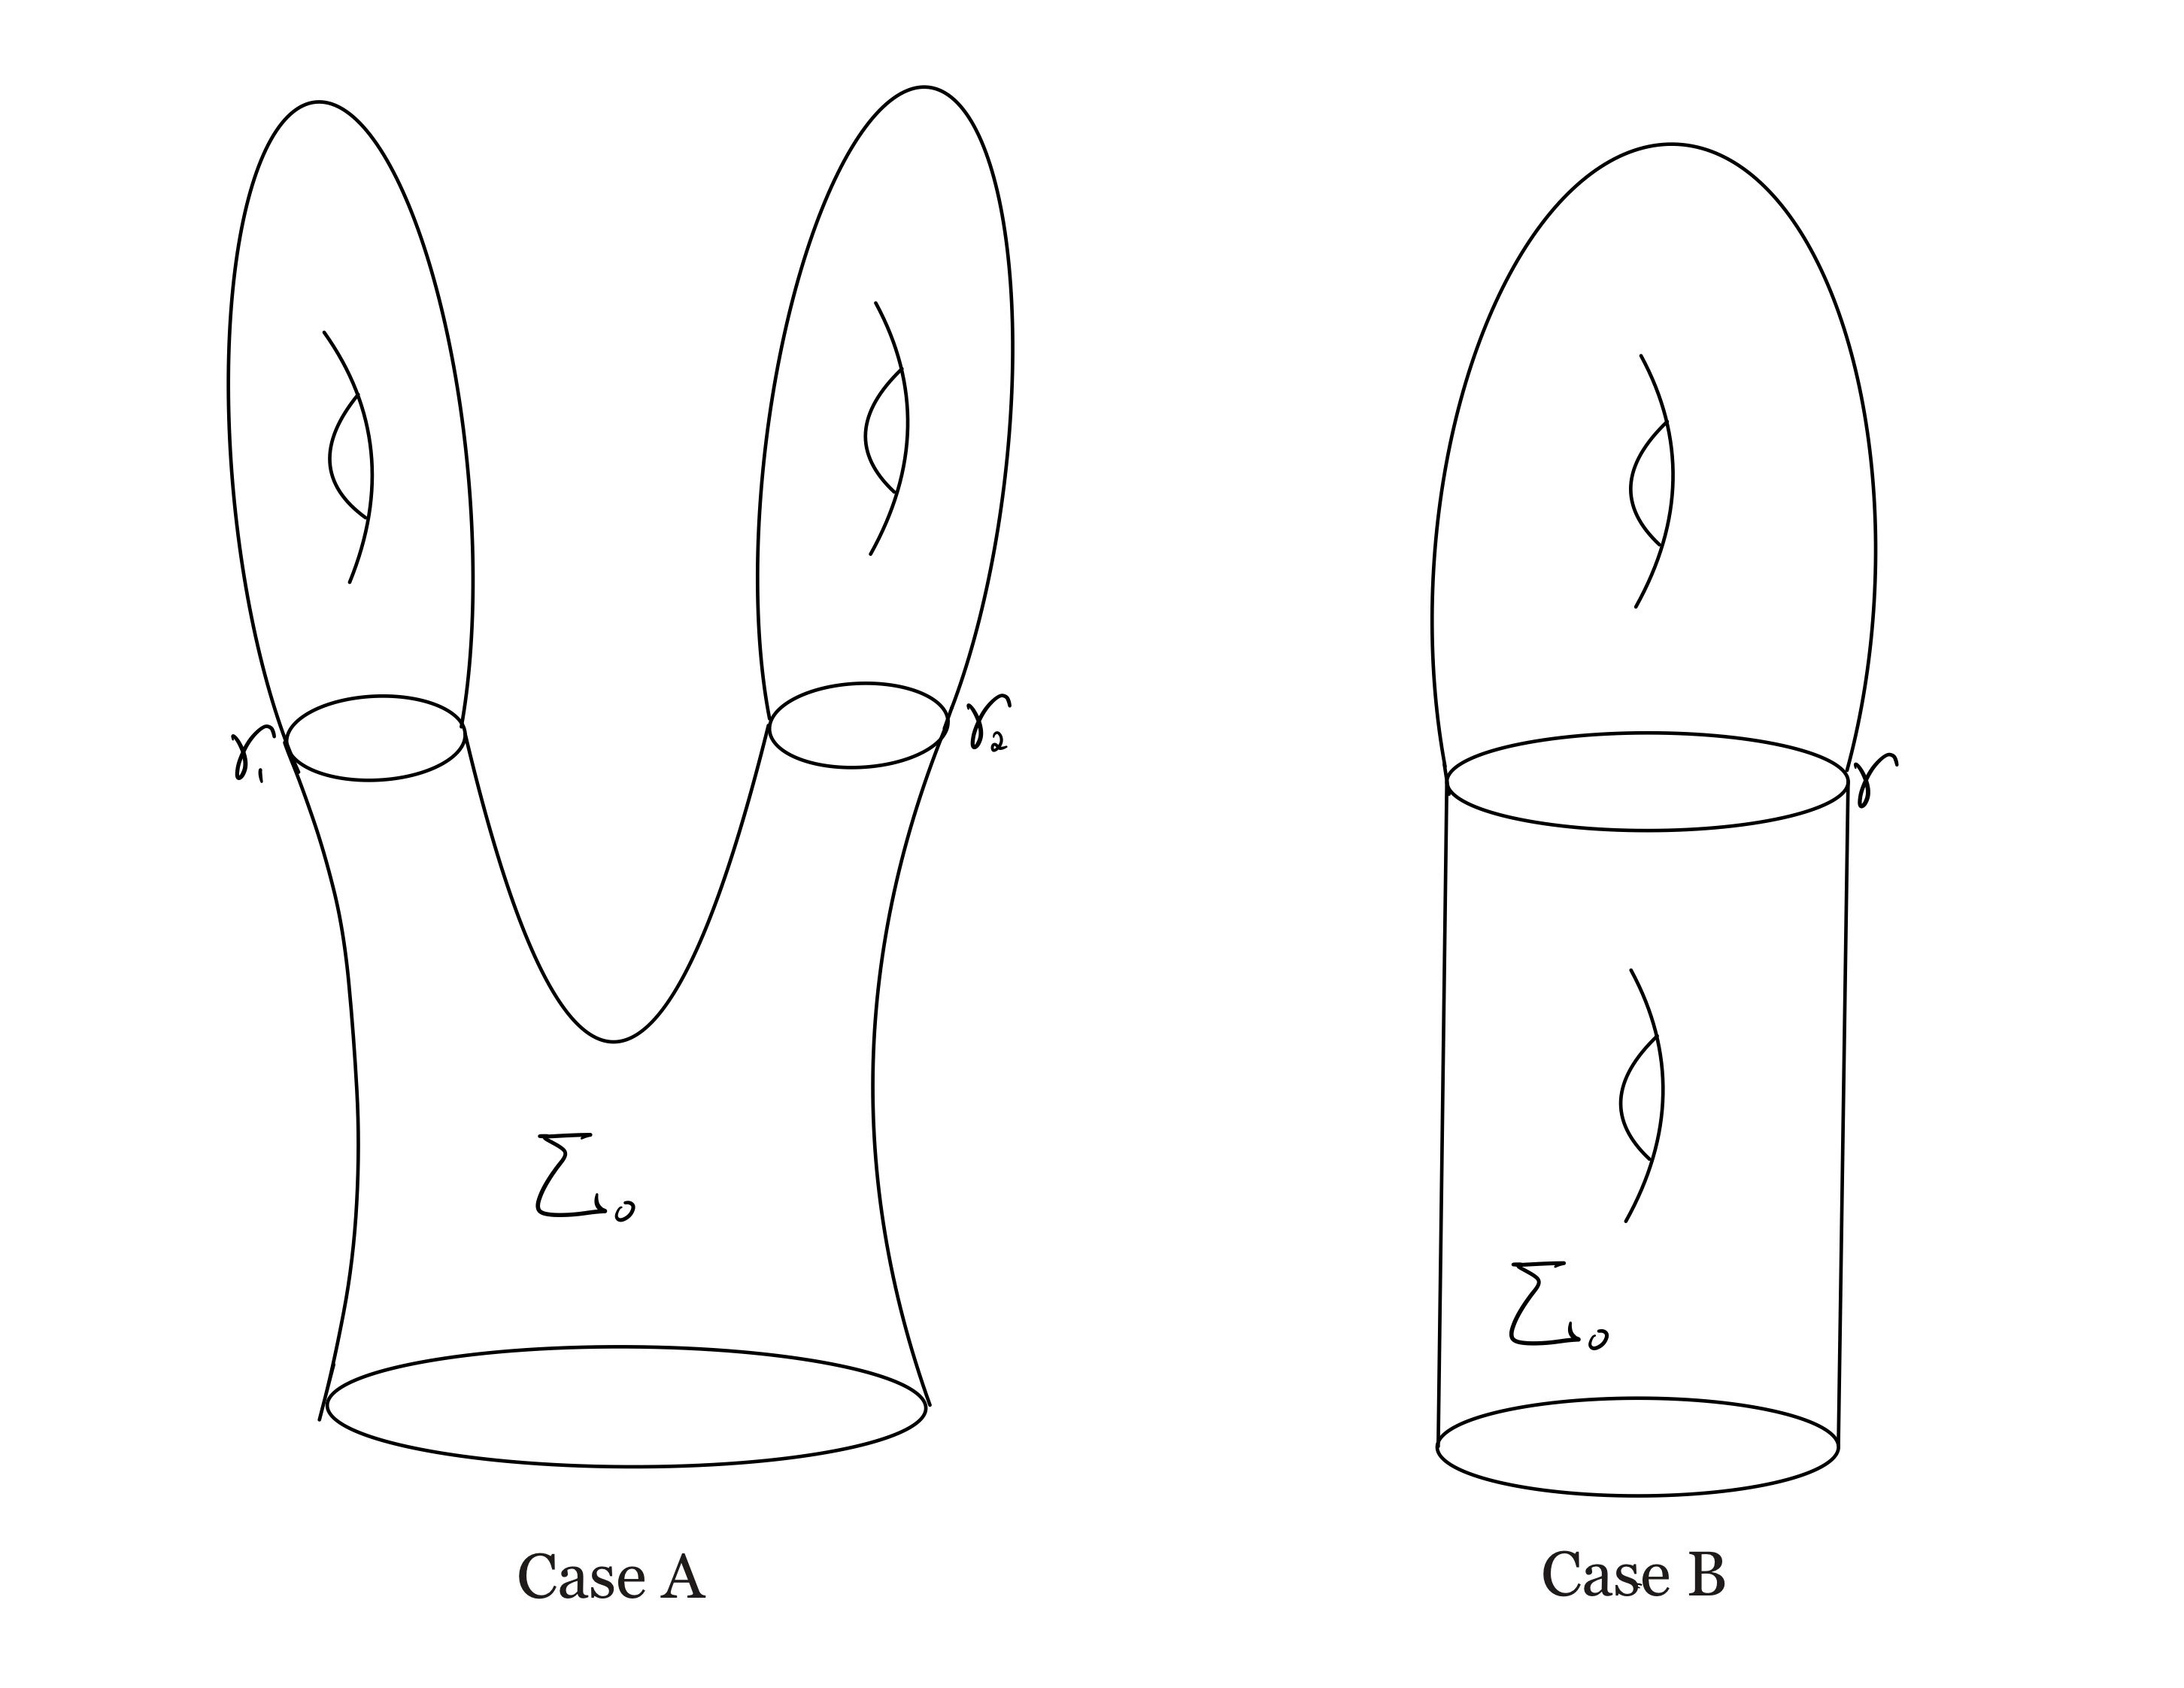
\includegraphics[width=\linewidth]{figures_satellite/Satellite Cases-1.jpg}
    \caption{The two non-trivial cases of $\Gamma$.}
    \label{fig:two_satellite_cases}
\end{figure}

\begin{myproof}
    By a result of Baldwin and Sivek \cite{BaldwinSivekInPrep}, for a fibered knot in an L-space, every curve in the canonical reducing system $\Gamma$ is separating. Furthermore, by definition, $\Gamma$ is a minimal collection of disjoint, essential, and non-boundary-parallel simple closed curves.

    The surface $\Sigma_2^1$ has genus $g=2$ and one boundary component $\partial \Sigma = K$. We analyze the possible components of $\Sigma_2^1 \setminus \Gamma$ based on the number of curves in $\Gamma$.

    Suppose $\Gamma \neq \emptyset$, and let $\gamma \in \Gamma$. Because $\gamma$ is separating, cutting $\Sigma_2^1$ along $\gamma$ yields two disconnected subsurfaces, $S_1$ and $S_2$. Since the original surface has exactly one boundary component $K$, exactly one of these subsurfaces must contain $K$. Let $S_1$ be the subsurface containing $K$, meaning $\partial S_1 = K \cup \gamma$. The other subsurface, $S_2$, has exactly one boundary component, $\partial S_2 = \gamma$.

    The sum of the genera of the subsurfaces must equal the genus of the original surface, so $g(S_1) + g(S_2) = g(\Sigma_2^1) = 2$. We can rigorously determine the genera of these pieces:
    \begin{itemize}
        \item Since $\gamma$ is an essential curve, it cannot bound a disk. Therefore, the one-boundary surface $S_2$ cannot be a disk, which strictly forces $g(S_2) \geq 1$.
        \item Since $\gamma$ is not boundary-parallel to $K$, the two-boundary surface $S_1$ cannot be an annulus. Therefore, $g(S_1) \neq 0$, which strictly forces $g(S_1) \geq 1$.
    \end{itemize}
    The only integer solution to $g(S_1) + g(S_2) = 2$ given these constraints is $g(S_1) = 1$ and $g(S_2) = 1$. Consequently, any single separating curve $\gamma \in \Gamma$ must decompose $\Sigma_2^1$ into $S_1 \cong \Sigma_1^2$ (a genus-one surface with two boundaries) and $S_2 \cong \Sigma_1^1$ (a once-punctured torus).

    We now classify $\Gamma$ by its size:

    \textbf{Case 1: $|\Gamma| = 1$.}
    If $\Gamma = \{\gamma\}$, the outermost component $\Sigma_0$ is precisely the subsurface containing $K$. As shown above, $\Sigma_0 = S_1 \cong \Sigma_1^2$. Thus, the outer surface is genus one with boundary components $K$ and $\gamma$. This corresponds exactly to \textbf{Case B}.

    \textbf{Case 2: $|\Gamma| = 2$.}
    Suppose $\Gamma = \{\gamma_1, \gamma_2\}$. The curves are disjoint, so $\gamma_2$ must lie entirely within $S_1$ or $S_2$ (defined by cutting along $\gamma_1$). It is a standard topological fact that a once-punctured torus ($\Sigma_1^1$) contains no essential, non-boundary-parallel separating curves; any separating curve on $\Sigma_1^1$ must bound a disk or be parallel to the boundary puncture. Therefore, $S_2$ cannot contain $\gamma_2$.

    Thus, $\gamma_2$ must lie inside $S_1$. Since $\gamma_2 \in \Gamma$, it is also a separating curve for the global surface $\Sigma_2^1$, meaning it must cut off another once-punctured torus ($\Sigma_1^1$) from $S_1$.
    By cutting the genus-one surface $S_1$ along $\gamma_2$, we subtract a genus-one piece, leaving a remainder of genus zero. This remaining outermost component $\Sigma_0$ now contains three boundaries: the knot $K$, the cut $\gamma_1$, and the cut $\gamma_2$. A genus-zero surface with three boundaries is a pair of pants ($\Sigma_0^3$). This corresponds exactly to \textbf{Case A}.

    \textbf{Case 3: $|\Gamma| \geq 3$.} If there were a third curve $\gamma_3$, it would have to reside within one of the components of $\Sigma_2^1 \setminus \{\gamma_1, \gamma_2\}$. Those components are two once-punctured tori and one pair of pants. None of these subsurfaces can contain an essential, non-boundary-parallel simple closed curve. Thus, $\Gamma$ can contain at most two curves.

    Therefore, up to homeomorphism, the only possibilities for $\Gamma$ are the empty set, Case A, or Case B.
\end{myproof}



The following Proposition of Baldwin-Sivek gives a classification result of $K$ when the outer map is periodic.

\begin{prop}[\cite{baldwin2025lspaces} Proposition 2.3] \label{prop:knottracesprop}
If $\phi_0$ is periodic, then either
    \begin{itemize}
        \item $\Gamma = \emptyset$ and $K$ is a $(p, q)$-torus knot, or
        \item $\Gamma  \neq \emptyset$ and either
        \begin{itemize}
            \item $K$ is a composite knot and $\Sigma_0$ is a planar surface, or
            \item $K$ is a $(p, q)$-cable knot of some other knot in $S^3$ and $\Sigma_0$ has genus $g(T_{p,q})$
        \end{itemize}
    \end{itemize}
    In each case above, $q \geq 2$ and $\gcd(p, q) = 1$.
\end{prop}

We isolate one further fact, relating the genus of the outermost piece to the genus of the pattern in the unknot. It underlies both the granny analysis below and the cable detection of Chapter \ref{chap:cable_detection}, and it is the hinge that determines which reducing-system configuration a given satellite occupies.

\begin{lemma}\label{lem:outer_genus_equals_pattern_genus}
Let $K = P(C)$ be a fibered satellite knot with companion solid torus $V$ and satellite torus $T = \partial V$, and suppose the pattern-in-the-unknot $P(U)$ is fibered. Let $\Sigma$ be the fiber of $K$, isotoped so as to meet $T$ in the minimal number of curves, which is then the wrapping number $m$ of $K$, and let $\Sigma_0 = \Sigma \cap V$ be the outermost piece, with boundary $\partial \Sigma_0 = K \cup (\Sigma \cap T)$. Then capping off the $m$ curves of $\Sigma \cap T$ with disks in the standardly embedded solid torus yields the fiber of $P(U)$, and this operation preserves genus, so
\[
g(\Sigma_0) = g(P(U)).
\]
\end{lemma}

\begin{proof}
Embed $V$ standardly in $S^3$, so that its core is unknotted. This is precisely the change of ambient space that carries the satellite $K = P(C)$ to the pattern-in-the-unknot $P(U)$, and it leaves the piece $\Sigma_0 \subset V$ unchanged. Under the standard embedding the curves $\Sigma \cap T$ bound meridional disks of the complementary solid torus; attaching these $m$ disks to $\Sigma_0$ produces a surface $\widehat{\Sigma}_0$ whose only boundary component is $K$. Since $K$ and $P(U)$ are fibered and the global monodromy preserves $T$, the surface $\widehat{\Sigma}_0$ is the fiber of $P(U)$.

Capping a surface with $m$ disks raises the Euler characteristic by $m$ while removing $m$ boundary components. Writing $\chi = 2 - 2g - b$ for a surface of genus $g$ with $b$ boundary components, and noting that $\Sigma_0$ has $b = m+1$ boundary components while $\widehat{\Sigma}_0$ has one,
\[
1 - 2g(\widehat{\Sigma}_0) = \chi(\widehat{\Sigma}_0) = \chi(\Sigma_0) + m = \bigl(1 - 2g(\Sigma_0) - m\bigr) + m = 1 - 2g(\Sigma_0),
\]
so $g(\widehat{\Sigma}_0) = g(\Sigma_0)$. Hence $g(\Sigma_0) = g(\widehat{\Sigma}_0) = g(P(U))$.
\end{proof}

We shall need one more proposition before we are ready to prove the main result of this chapter.

\begin{prop}\label{prop:capping_trefoil}
    Let $K = P(C)$ be a fibered satellite knot with Seifert genus $g(K) = 2$ and algebraic winding number $w=1$, where the companion $C$ and the pattern knot in the unknot $P(U)$ are both trefoils. Let $h \colon \Sigma \to \Sigma$ be the monodromy of $K$.
    Suppose the Nielsen-Thurston form of $h$ is Case B as in Lemma \ref{lem:satellite_CaseACaseB}. The outer map
    \[
    \phi_0 \colon \Sigma_0 \to \Sigma_0
    \]
    can be capped off at the boundary component $\gamma$ with a disk. The resulting map on the surface $\widehat{\Sigma}_0 \cong \Sigma_1^1$:
    \[
    \widehat{\phi}_0 \colon \widehat{\Sigma}_0 \to \widehat{\Sigma}_0
    \]
    is precisely the monodromy of the trefoil $P(U)$.
\end{prop}

\begin{proof}
    Let $V$ be the solid torus containing the pattern $P$, and let $T = \partial V$ be its boundary. In the satellite construction, $V$ is embedded in $S^3$ such that its core is the companion knot $C$. The boundary $T$ forms an essential JSJ torus in the knot exterior.

    Let $m$ be the wrapping number of $K$. By Schubert's geometric genus inequality (Theorem \ref{thm:schubert}), the genera must satisfy
    \[
    g(K) \geq g(P(U)) + m \cdot g(C).
    \]
    Substituting our known values yields $2 \geq 1 + m \cdot 1$, which simplifies to $m \leq 1$. However, by definition, the geometric wrapping number must be at least the absolute value of the algebraic winding number, so $m \geq |w| = 1$. These two inequalities strictly force the geometric wrapping number to be $m = 1$. Consequently, the fiber surface $\Sigma$ can be isotoped to intersect the JSJ torus $T$ in exactly one simple closed curve, which is our Thurston reducing curve $\gamma$.

    This curve $\gamma$ splits $\Sigma$ into two compact subsurfaces. By our convention, the ``outer'' surface $\Sigma_0 = \Sigma \cap V$ resides entirely inside the solid torus. Its boundary consists of exactly two components: $\partial \Sigma_0 = K \cup \gamma$.

    We construct a new surface by capping off strictly the boundary component $\gamma$. Abstractly, we attach a 2-disk $D^2$ to $\gamma$, forming the surface
    \[
    \widehat{\Sigma}_0 = \Sigma_0 \cup_{\gamma} D^2.
    \]
    The only remaining boundary of this new surface is the knot $K$.

    Capping off $\gamma$ in this abstract way corresponds, geometrically, to changing the ambient 3-manifold. The curve $\gamma$ is a longitude of $V$ --- it lies on $T = \partial V$ and runs once longitudinally around the solid torus. Inside $V$, the curve $\gamma$ does not bound a disk (it is essential in $\pi_1 V$), so the capping disk cannot live inside the original $S^3$. Instead, the capping operation corresponds to \emph{unknotting} the companion: we replace the knotted complement $S^3 \setminus \mathring{V}$ with a standardly embedded solid torus, which has a meridional disk whose boundary is precisely the relevant longitude. Equivalently, this is the change of ambient space that takes the satellite knot $K = P(C)$ to the pattern-in-the-unknot $P(U)$.

    Under this change of ambient space, the embedding of $V$ becomes standard, and the satellite knot $K = P(C)$ is transformed into the pattern knot in the unknot, $P(U)$. Therefore, the capped-off surface $\widehat{\Sigma}_0$ is a Seifert surface for $P(U)$. By Lemma \ref{lem:outer_genus_equals_pattern_genus}, $g(\Sigma_0) = g(P(U)) = 1$, so $\widehat{\Sigma}_0$ is exactly the minimal-genus fiber of the trefoil $P(U)$.

    The global monodromy $h$ preserves the JSJ torus $T$ and thus restricts to an automorphism
    \[
    \phi_0 \colon \Sigma_0 \to \Sigma_0
    \]
    that fixes both boundary components $K$ and $\gamma$ pointwise.

    When we cap off $\gamma$ with the disk $D^2$, the homeomorphism $\phi_0$ extends naturally to the disk by the identity, yielding a well-defined homeomorphism $\widehat{\phi}_0 \colon \widehat{\Sigma}_0 \to \widehat{\Sigma}_0$ that fixes the boundary $K$.

    Because capping off $\gamma$ unties the companion and transforms the ambient fibration into the standard fibration of the unknotted solid torus, this extended map $\widehat{\phi}_0$ is precisely the geometric monodromy of the resulting knot. Since $P(U)$ is a trefoil, $\widehat{\phi}_0$ is the geometric monodromy of the trefoil.
\end{proof}

We are now ready to prove the main result of this chapter, Theorem \ref{theorem:satellite}.

\begin{myproof}[Proof of Theorem \ref{theorem:satellite}]
    By Theorem \ref{theorem:ni-fibered}, $K$ is fibered; and by Equation \ref{eq:ozvath-szabo genus top grading}, of genus two. Let
    \[
    h \colon \Sigma_2^1 \to \Sigma_2^1
    \]
    be the monodromy of $K$. Let $(\phi_h,\Gamma)$ be the Nielsen-Thurston form of the monodromy.

    If $\Gamma = \emptyset$, then $\Sigma_0 = \Sigma_2^1$, and
    \[
    \phi_0 \colon \Sigma_0 \to \Sigma_0.
    \]
    is periodic. Otherwise, $K$ would be a hyperbolic knot, and not a satellite knot by Theorem \ref{theorem:thurston classification of knots}. Hence Proposition \ref{prop:knottracesprop} applies, in particular $K$ is a $(p,q)$-torus knot. However, the knot Floer homology of torus knots is well-known, and none coincides with that of $T(2,3) \# T(2,3)$. Specifically, all torus knots are L-space knots (or mirrors of L-space knots). A defining property of L-space knots is that the rank of their knot Floer homology in any fixed Alexander grading $a$ is at most $1$. Thus, if $K = T_{p,q}$, then
    \[
    \widehat{HFK}(T(2,3)\#T(2,3)) \cong \widehat{HFK}(K) \cong \widehat{HFK}(T(p,q)),
    \]
    and we must have
    \[
    \operatorname{rank} \widehat{HFK}(K, a) \le 1
    \]
    for all $a \in \mathbb{Z}$. But this is a contradiction, as it is known that the rank of the second-to-top Alexander grading of $\widehat{HFK}(T(2,3)\#T(2,3))$ is $2$.

    Hence $\Gamma \neq \emptyset$, and this can be either Case A or Case B, by Lemma \ref{lem:satellite_CaseACaseB}.

    Suppose the fiber $\Sigma_2^1$ and its reducing system is of Case A. Then $\Sigma_0$ is homeomorphic to a pair of pants, which is known to not support pseudo-Anosov homeomorphisms (see, e.g., Farb-Margalit\cite{farb2012primer}). This follows from the observation that every essential simple closed curve on the pair of pants is boundary-parallel; thus, every homeomorphism preserves a multicurve (the boundary itself) and is therefore reducible. Hence in this case $\phi_0 \colon \Sigma_0 \to \Sigma_0$ must be periodic, thus Proposition \ref{prop:knottracesprop} applies, specifically the case for when $\Gamma \neq \emptyset$.

    Consider first the cable knot sub-case, i.e., that $K$ is a $(p,q)$-cable knot. A cable knot has winding number at least $2$: its pattern is a non-trivial torus knot on $\partial V$, whose longitudinal wrapping is the parameter $q \geq 2$ of Proposition \ref{prop:knottracesprop}. This contradicts Lemma \ref{lem:satellite_trefoils_windingnumber_1}, which forces the winding number of $K$ to be $1$. Hence the cable sub-case cannot occur. (We note for contrast that this is precisely the configuration occupied by the $(2,1)$-cable $C_{2,1}(T_{2,3})$ of Chapter \ref{chap:cable_detection}, whose winding number is $2$; it is excluded here only because the granny target forces winding number $1$.)

    Thus it must be the sub-case that $K$ is a composite knot. In other words, $K$ is a genus-two satellite knot that is a connect-sum of two genus-one knots. The only genus-one knots are the trefoils and the figure-eight knot. The Alexander polynomial of the connect-sum of one of the trefoils (either the left- or right-handed) and the figure-eight knot is the product of their respective Alexander polynomials:
    \begin{align*}
        \Delta_{3_1 \# 4_1} (t)&= \Delta_{\bar{3}_1 \# 4_1}(t)\\
        &= \Delta_{3_1}(t) \cdot \Delta_{4_1}(t)\\
        &= (t - 1 + t^{-1})\cdot (-t +3 -t^{-1})\\
        &= -t^2 + 4t - 5 + 4t^{-1} - t^{-2}.
    \end{align*}

    Which differs from that of $T(2,3)\#T(2,3)$, hence that of $K$. Therefore, $K$ must be the connect-sum of trefoils, and it must be in fact the connect-sum of the right-handed trefoils since the $\widehat{HFK}$ of the square knot $\overline{T(2,3)}\# T(2,3)$ and of $\overline{T(2,3)} \# \overline{T(2,3)}$ both differ from
    \[
    \widehat{HFK}(T(2,3) \# T(2,3)) \cong \widehat{HFK}(K)
    \]
    as bigraded vector spaces.

    Now suppose that the fiber $\Sigma_2^1$ and its reducing system is of Case B. There are two possibilities: either the outermost map $\phi_0$ is periodic, or it is pseudo-Anosov.

    Suppose $\phi_0$ is periodic. Then since $\Gamma \neq \emptyset$ and $\Sigma_0$ is not planar, Proposition \ref{prop:knottracesprop} implies that $K$ is a $(p,q)$-cable knot of a knot in $S^3$ and $\Sigma_0$ has genus $g(T_{p,q})$, where $q\geq 2$ and $\gcd(p,q) = 1$. Since $\Sigma_0$ of Case B has genus one, we have
    \[
    g(\Sigma_0) = g(T_{p,q}) = 1.
    \]
    The only genus one torus knots are the trefoils, hence $K$ is a cable knot with trefoil pattern, where the trefoils are embedded in the solid torus as torus knots (as required by the definition of a cable knot). However, this is a contradiction, as the presentation of the trefoils as torus knots yields winding number 2 if presented as $T(2,3)$ on the solid torus, and winding number 3 if presented as $T(3,2)$ on the solid torus. This contradicts Lemma \ref{lem:satellite_trefoils_windingnumber_1} which states that the winding number of $K$ must be 1.

    So suppose $\phi_0$ is pseudo-Anosov. Then Proposition \ref{prop:knottracesprop} does not apply. However, from Lemma \ref{lem:satellite_trefoils_windingnumber_1}, it is still known that $K = P(C)$ satisfies $P(U)$ and $C$ are trefoils, and the winding number $w$ is 1.

    Let us consider the capped-off map
    \[
    \widehat{\phi}_0 \colon \widehat{\Sigma}_0 \to \widehat{\Sigma}_0
    \]
    of $\phi_0$. That is, capping off $\Sigma_0$ along $\Gamma = \gamma$ with a disk and extending $\phi_0$ to the identity along the capping disk to obtain $\widehat{\phi}_0$. This map is in fact the monodromy of the trefoil $P(U)$ by Proposition \ref{prop:capping_trefoil}, which is known to be not pseudo-Anosov (since the trefoils are not hyperbolic). Consequently, the number of prongs on $\Sigma_0$ located at $\Gamma$ must be 1. Otherwise, the capped off map would still be pseudo-Anosov. We claim that on the other boundary component, which we denote by $\partial \Sigma$, there is also only one prong. Indeed, the map $\phi_0$ commutes with the hyperelliptic involution $\iota$. By construction, $\iota$ exchanges the two boundary components of $\Sigma_0$. Since $\iota$ is a diffeomorphism preserving the invariant foliation, it must map the singularity at $\Gamma$ to the singularity at $\partial \Sigma$. Consequently, the number of prongs at both boundaries must be identical.

    This implies that the fractional Dehn twist coefficient $c(K)$ is at least one and an integer:
    \[
    |c(K)| \geq 1, \quad |c(K)| \in \mathbb{Z}.
    \]
    On the other hand, since $K$ is a fibered knot in $S^3$ and $S^3$ is an L-space, the theorem of Hedden and Mark\cite{hedden2018floer} bounds the fractional Dehn twist coefficient by
    \[
    |c(K)| \leq 1.
    \]
    Therefore, the only possibility is
    \[
    |c(K)| = 1.
    \]
    We show that this is not possible. Suppose by way of contradiction that
    \[
    c(K) = 1.
    \]
    Let $-Y$ denote the manifold defined by the open book decomposition $(\Sigma_2^1, \phi_h)$, which must be $S^3$, with reverse orientation:
    \[
    -Y = -Y_{(\Sigma_2^1,\phi_h)} \cong S^3.
    \]
    Let $-Y_1(K)$ denote the result of performing $1$-surgery along the binding $K$ on $-Y$, and let $-Y_0(K)$ denote the result of performing $0$-surgery. The $1$-surgery is equivalent to the open book decomposition obtained by composing $\phi_h$ with a right-handed Dehn twist along the boundary:
    \[
    -Y_1(K) \cong -Y_{(\Sigma_2^1,\phi_h \circ T_\partial)}.
    \]
    Let $\xi_1$ denote the contact structure on $-Y_1(K)$ supported by this open book.

    The triple $(-Y_1(K),-Y,-Y_0(K))$ fits into a surgery exact triangle of Ozv\'{a}th-Szab\'{o}, with twisted coefficients on the $0$-surgery term (cf.\ Hedden-Mark\cite{hedden2018floer}, Section 5):
    \[
    \dots \longrightarrow HF^+(-Y_1(K);\mathbb{F}) \xlongrightarrow{H} HF^+(-Y;\mathbb{F}) \xlongrightarrow{G} HF^+(-Y_0(K);\mathbb{F}[C_1]) \xlongrightarrow{F} HF^+(-Y_1(K);\mathbb{F}) \longrightarrow \dots
    \]
    All maps in this triangle are $\mathbb{F}[U]$-equivariant, where $U$ is the formal variable of degree $-2$ in the $\mathbb{F}[U]$-module structure on $HF^+$.

    We focus on the canonical spin$^c$ structure $\mathfrak{s}_{1-g}$ on $-Y_0(K)$, namely the one cobordant through the surgery cobordism to $\mathfrak{s}_{\xi_1}$ and satisfying $\langle c_1(\mathfrak{s}_{1-g}), [\widehat{S}]\rangle = 2-2g$ on the capped-off fiber. By Lemma 2.1 of Hedden-Mark\cite{hedden2018floer}, the corresponding summand satisfies
    \[
    HF^+(-Y_0(K), \mathfrak{s}_{1-g}; \mathbb{F}[C_1]) \cong \mathbb{F}[C_1] \cong \mathbb{F},
    \]
    on which $U$ acts as zero.

    Let $G_{1-g}$ and $F_{1-g}$ denote the components of $G$ and $F$ corresponding to this summand:
    \[
    HF^+(-Y; \mathbb{F}) \xlongrightarrow{G_{1-g}} \mathbb{F} \xlongrightarrow{F_{1-g}} HF^+(-Y_1(K), \mathfrak{s}_{\xi_1};\mathbb{F}).
    \]

    \textbf{Claim:} The map $G_{1-g}$ is zero.

    \textit{Proof of claim.} Since $-Y \cong S^3$ is an L-space (indeed, the simplest one),
    \[
    HF^+(-Y; \mathbb{F}) \cong \mathcal{T}^+ := \mathbb{F}[U, U^{-1}]\big/U \cdot \mathbb{F}[U],
    \]
    the tower module. On $\mathcal{T}^+$, the action of $U$ is \emph{surjective}: for every $U^{-k} \in \mathcal{T}^+$ with $k \geq 0$, we have $U \cdot U^{-(k+1)} = U^{-k}$. Therefore, every element $x \in HF^+(-Y)$ may be written as $x = U \cdot y$ for some $y \in HF^+(-Y)$. By $\mathbb{F}[U]$-equivariance of $G_{1-g}$ and the fact that $U$ acts as zero on the target $\mathbb{F}$,
    \[
    G_{1-g}(x) = G_{1-g}(U \cdot y) = U \cdot G_{1-g}(y) = 0.
    \]
    Hence $G_{1-g} \equiv 0$, as claimed. \hfill$\square$

    By exactness of the surgery triangle restricted to the $\mathfrak{s}_{1-g}$ summand,
    \[
    \ker(F_{1-g}) = \operatorname{im}(G_{1-g}) = 0,
    \]
    so $F_{1-g}$ is injective. Since its source $\mathbb{F}$ is non-zero, $F_{1-g}$ is non-trivial.

    By Proposition 2.4 of Hedden-Mark\cite{hedden2018floer}, non-triviality of $F$ on the $\mathfrak{s}_{1-g}$ summand implies that the contact invariant
    \[
    c(\xi_1) \in HF^+(-Y_1(K); \mathbb{F})
    \]
    is non-zero. By Theorem 1.4 of Ozv\'{a}th-Szab\'{o}\cite{ozsvath2004holomorphic}, this implies that $\xi_1$ is \emph{tight}.

    On the other hand, by assumption $c(\phi_h) = 1$, so composition with a right-handed boundary Dehn twist gives
    \[
    c(\phi_h \circ T_\partial) = 0.
    \]
    Since $\phi_h \circ T_\partial$ is pseudo-Anosov and has vanishing fractional Dehn twist coefficient on its (single) boundary component, Proposition 3.1 of Honda-Kazez-Mati\'c\cite{honda2007right} implies that $\phi_h \circ T_\partial$ is \emph{not} right-veering. By Theorem 1.1 of the same paper, the contact structure $\xi_1$ supported by $(\Sigma_2^1, \phi_h \circ T_\partial)$ is therefore \emph{overtwisted}, contradicting the tightness established above.

    For the case of
    \[
    c(K) = -1,
    \]
    the same argument works with $Y$ in place of $-Y$, and a left-handed Dehn twist in place of the right-handed Dehn twist.
\end{myproof}
\begin{remark}
The satellite analysis above eliminates every candidate for $K$, and we have not had occasion to consider the $(2,1)$-cable of the right-handed trefoil, $C_{2,1}(T_{2,3})$, as a candidate: Lemma \ref{lem:satellite_trefoils_windingnumber_1} already excludes it on two counts (its winding number is $2$, not $1$, and its pattern $P(U) = T_{2,1}$ is the unknot rather than a trefoil). Nevertheless, $C_{2,1}(T_{2,3})$ is itself a fibered satellite knot of genus two, and one may ask whether its knot Floer homology is detected by $\widehat{HFK}$ in the same spirit as our main theorem. We establish a corresponding detection result for $C_{2,1}(T_{2,3})$---namely, that any knot $K' \subset S^3$ with $\widehat{HFK}(K'; \mathbb{F}) \cong \widehat{HFK}(C_{2,1}(T_{2,3}); \mathbb{F})$ and satisfying additional hyperbolic-monodromy hypotheses must in fact be $C_{2,1}(T_{2,3})$---in Chapter \ref{chap:cable_detection}.
\end{remark}
